\chapter{Metodología}

En el presente capítulo se detallarán las etapas y procesos necesarios del sistema para lograr la estimación de la mirada de las personas, esto incluye desde los métodos para el cálculo de los ángulos de mirada de las personas a un objeto en específico, el proceso de generación y selección de las marcas en el piso donde se colocan las personas y las marcas en la pantalla, el proceso de optimización numérica, estimación del plano del piso y finalmente la red neuronal y como se implementa.

 \section{Descripción general del sistema}
 El sistema de estimación de la mirada que se propone en este proyecto de tesis funciona para posiciones discretas de lo que se observa, es decir, se estiman regiones del plano enfrente de las personas. La estructura del sistema ya calibrado y funcionando consta de 3 etapas: 
 \begin{itemize}
 	\item Detección del rostro.- Se utiliza el algoritmo detector de rostros de Viola y Jones para localizar el rostro de la persona en la imagen.
 	\item Extracción de características del rostro.- Se extraen las características 3d del rostro que incluyen la posición en 3d, y las características de la imagen que ayudan al clasificador
 	\item Clasificador.- Se encarga de producir en la salida una región en la pantalla que representa lo que está observando la persona detectada en etapas previas, el algoritmo es una red neuronal artificial de retropropagación entrenada con anterioridad.
 \end{itemize}
\begin{figure}[htbp]
	\centering
	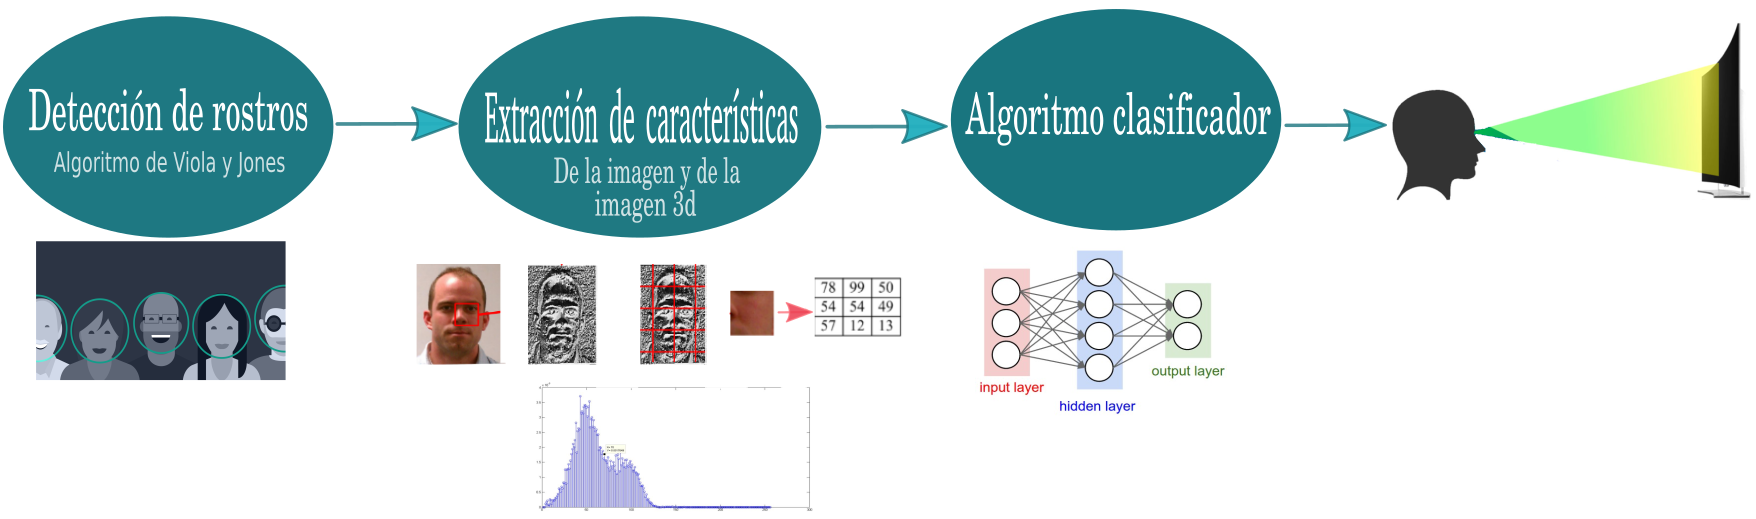
\includegraphics[width=1\textwidth]{./pictures/etapas}     	
\end{figure}
 Una de las etapas cruciales de este proyecto es la captura precisa de datos, entre esos datos está la ubicación del rostro en tres dimensiones en la escena, para lograr lo anterior se debe conocer el plano del piso en el que las personas habitan, esto es, la ecuación matemática que describe dicho plano, el cual se obtiene a partir de la estimación de la matriz de rotación y traslación que tiene la cámara con respecto al piso. Además en este capítulo se detalla como implementar el algoritmo de Levenberg-Marquardt para optimizar la matriz de rotación y traslación. Otro apartado importante de la metodología incluye determinar en cuales  puntos del piso \sout{en los que vale la pena} que se coloquen las personas para capturar sus datos. 
 Finalmente se describe como se realiza la implementación de la red neuronal teniendo con las imágenes de los rostros y los datos 3d como vector de características.
 A continuación en la metodología se describen las herramientas y técnicas necesarias para estimar la ecuación del plano.

    \section{Mapeo de coordenadas a ángulos}
    Uno de los problemas que hay que tomar en cuenta y definir en el presente trabajo antes de realizar los experimentos, es describir la relación que existe entre la ubicación en metros de lo que está mirando el sujeto de estudio en la pantalla y la pose de la cabeza de esta persona medida en ángulos, tomando en cuenta diversos aspectos como: la estatura de la persona, la distancia de la persona a la pantalla, cuál es el marco de referencia, etc. Esta sección consiste en describir cómo se realiza el mapeo (o la ecuación) de dicho objeto desplegado en pantalla y la orientación de la cabeza, primero se describirá la geometría del escenario. 
    \begin{figure}[htbp]
    	\centering
    	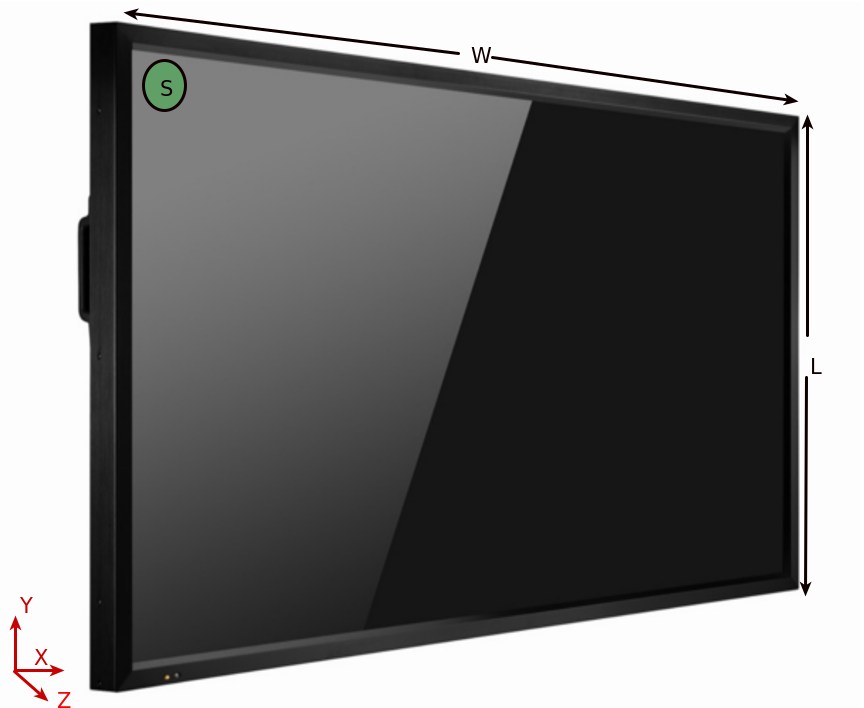
\includegraphics[width=0.5\textwidth]{./pictures/pantalla2}
    	\caption{}\label{fig: figura}
    \end{figure}   
    \\La pantalla que observa el sujeto del experimento se coloca en una pared a una distancia de $L_y$ metros del piso, la pantalla tiene unas dimensiones de $W$ m. de ancho y $L$ m. de alto. El sistema de coordenadas tiene su origen en la cámara y se ubica  encima de la pantalla y a la mitad del ancho W, \textbf{la recta que se encuentra a lo largo de W es paralela al eje $X$ y la que está a lo largo de L es paralela a $Y$}. Las personas se encontrarán paradas en un mismo plano (piso) y enfrente de la pantalla a una distancia $D_z$. Hay un punto en específico del rostro de las personas que es de interés y es el que se utiliza para realizar el análisis, este punto se define como $P$ y se encuentra a la mitad de la linea que une los ojos. El vector $\vec v$ sale del punto $P$ y es ortogonal al plano de la cara, el punto $P$ se encuentra a una distancia $H_y$ con respecto al piso y es dependiente de la estatura de la persona. Otro parámetro que se debe mencionar es el que hace referencia a la distancia que hay entre la persona y el origen sobre el eje $X$, es decir, la componente $X$ del punto $P$ de la persona y lo denotaremos como $a$.%La recta imaginaria que une el punto $P$ con el piso es $L_p$ y es perpendicular al plano del piso y por la misma razón es paralela al eje $Y$.
    \begin{figure}[htbp]
    	\centering
    	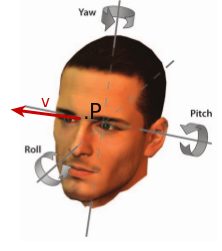
\includegraphics[width=0.36\textwidth]{./pictures/personaMirando}
    	\caption{}\label{fig: figura}
    \end{figure}
    
    Como se puede observar en la figura 1.2 las personas tenemos tres tipos de movimiento de la cabeza: yaw, pitch y roll; sin embargo para el análisis de este proyecto solo se toman en cuenta el movimiento de yaw y pitch, ya que estos son los movimientos que se dan cuando una persona mueve su cabeza para observar el objeto en dos dimensiones de la pantalla.\\
    El objeto de la pantalla que la persona observa es representado como $S$ y el vector $\vec v$ representa la mirada de la persona o lo que es lo mismo $\vec{PS}$, cuando la persona se encuentre mirando $S$ el vector $\vec v$  debe apuntar a $S$, esto quiere decir que si se proyecta el vector sobre la misma dirección hacia la pantalla debe intersectar $S$.\\
    El objeto $S$ se desplazará a través de toda la pantalla $(X,Y)$ metros, tomando como marco de referencia la esquina superior izquierda de la pantalla, a esta esquina le corresponde la coordenada $(0,0)$, $(X,Y)$ es la esquina inferior derecha y $(\frac{X}{2}, \frac{Y}{2})$ el centro de la pantalla.
    La pose de la cabeza se mide mediante dos ángulos: $\phi_x$ y $\phi_y$.
    \begin{itemize}
    	\item $\phi_y$.- Observando desde el plano $Y-Z$ representa que tanto se desvía el vector $\vec v$% sobre la recta $D_z$ que hay entre la persona y la pantalla.
    	\item $\phi_x$.- Observando desde el plano $X-Z$ (desde arriba de la persona y la pantalla) representa que tanto se desvía el vector $\vec v$ %sobre la recta $D_z$.
    \end{itemize}
    De igual manera el ángulo $\phi_x$ indica el movimiento yaw que la persona realiza al mirar como se traslada el objeto $S$ y el ángulo $\phi_y$ el movimiento pitch.
    
    \section{Ecuaciones de la mirada}
    Una vez definido el escenario y los aspectos a tomar en cuenta, ahora falta demostrar cual es la relación que se puede hallar entre la posición del objeto en la pantalla y la pose de la cabeza mediante los ángulos $\phi_x$ y $\phi_y$.
    
    \subsection{Desviación de $\phi_y$ y $\phi_x$. Primer caso}
    Para facilitar el análisis en esta sección se ilustra el escenario con todos los elementos en la figura 2.1
    \begin{figure}[htbp]
    	\centering
    	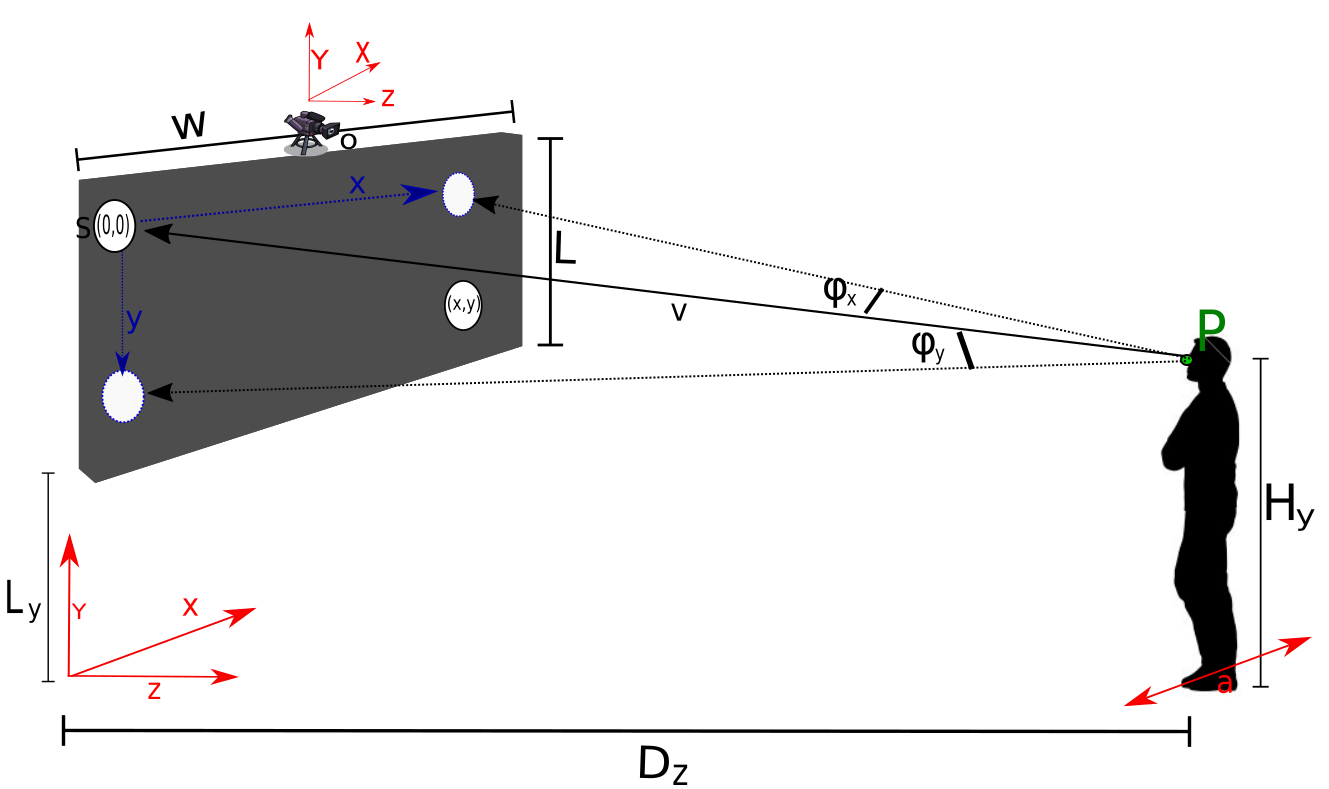
\includegraphics[width=0.7\textwidth]{./pictures/escenario}
    	\caption{Escenario y aspectos a tomar en cuenta}\label{fig: figura}
    \end{figure}
    \\Este caso es suponiendo que la cámara está colocada sobre la pantalla de tal forma que su eje $Z$ es paralelo al piso, esto quiere decir que el eje $Y$ de la cámara yace sobre el plano de la pantalla.\\
     El análisis comienza observando la escena desde el plano $Y-Z$, primero se definen dónde se encuentran con respecto al sistema de coordenadas los puntos más importantes, los cuales son: $S$ y $P$. Supongamos que el objeto a observar está en la coordenada $(x,y)$ de la pantalla, como se había mencionado previamente el sistema de coordenadas se encuentra centrado en la cámara,  a la mitad de la pantalla con respecto al eje $X$ y a una pequeña altura $c_y$ m. con respecto al eje y, el movimiento de $S$ yace sobre el plano $X-Y$ por lo que su componente en $z$ es igual cero, entonces:
    
    \begin{eqnarray}
    S= [S_x, S_y, S_z]^T= [x-W/2, -(c_y+y), 0]^T
    \end{eqnarray}
    Para hallar las componentes de P se toma la distancia $D_z$ a la que se encuentra del origen sobre el eje $Z$, como se había mencionado la persona se desplaza $a$ m sobre el eje $X$ y se encuentra a una distancia sobre el eje y de $L_y+L-H_y$:
    \begin{eqnarray}
    P=[P_x, P_y, P_z]^T= [a, -(L_y+L-H_y), D_z]^T
    \end{eqnarray}
  Ahora que ya se definieron donde se encuentran los puntos que se utilizarán con respecto al marco de referencia centrado en la cámara, se necesitan los ángulos entre la posición del vector $\vec v=\vec {PS}$ y cada uno de los ejes que son de interés, estos ángulos se conocen como cosenos directores del vector $\vec v$ y únicamente son necesarios los que se forman con el eje $Y$ y el $X$.
  Las fórmulas de los cosenos directores son:
  \begin{eqnarray}
  cos(\phi_y)=\frac{\vec v_y}{|\vec v|}\\
  cos(\phi_x)=\frac{\vec v_x}{|\vec v|}
  \end{eqnarray}
  
  donde $|\vec v|$ se halla mediante:
  \begin{eqnarray}
  \sqrt{\vec v_{x}^2+\vec v_{y}^2+\vec v_{z}^2}=\sqrt{(x-\frac{W}{2}-a)^2+(-c_y-y+(L_y+L-H_y))^2+(-D_z)^2}
  \end{eqnarray}
  \\Por lo tanto los ángulos de desviación son:
  
  \begin{eqnarray}
  \phi_y=cos^{-1} (\frac{-c_y-y+(L_y+L-H_y)}{\sqrt{(x-\frac{W}{2}-a)^2+(-c_y-y+(L_y+L-H_y))^2+(-D_z)^2}})\\
  \phi_x=cos^{-1}(\frac{x-\frac{W}{2}-a}{\sqrt{(x-\frac{W}{2}-a)^2+(-c_y-y+(L_y+L-H_y))^2+(-D_z)^2}})
  \end{eqnarray}   

      \subsection{Desviación de $\phi_y$ y $\phi_x$. Segundo caso}
      El segundo caso para calcular $\phi_y$ y $\phi_x$ es un tanto similar al primero pero con la diferencia de que para obtener dichos ángulos no es necesario que la cámara (origen) se encuentre en una rotación específica (paralela al piso) como en el caso anterior. Ahora los ángulos se calculan de manera independiente a la orientación de la camára, para lograr lo anterior únicamente se necesita conocer cual es la ecuación del piso con respecto a la cámara, la ubicación de la persona en el plano y su estatura. En las secciones siguientes se explica como se obtienen los parámetros del plano del piso $n$ (normal del plano) y $d$ (distancia más cercana al origen) mediante técnicas de visión computacional y geometría proyectiva.\\

      %Poner un poco de info de cosenos directores en el marco
      \subsubsection{Localización de P}
	    Como se mencionó anteriormente para hallar la mirada de las personas en los dos ángulos únicamente se necesita aplicar la fórmula de cosenos directores al punto $P$ (cabeza de la persona) y $S$ (objeto en pantalla).
      Sea $F=[F_x, F_y, F_z]$ un punto que yace en el piso donde se coloca la persona. $F$ se puede obtener estableciendo dos valores en la ecuación del plano, uno en el eje $x$ y el otro en el eje $z$ y el valor de $y$ se consigue despejando el la variable $y$ de la ecuación:
        \begin{eqnarray}
        y=\frac{d-Ax-Cz}{B}
        \end{eqnarray}
      De la ecuación anterior $F_x=x$, $F_y=y$ y $Fz=z$. Para encontrar $P$ simplemente se parte de $F$ y multiplicamos la estatura de la persona $H_y$ en dirección negativa (regla de la mano derecha) por la norma de la normal del plano, lo anterior se debe a que las personas al estar paradas sobre el piso siempre están paradas de una manera ortogonal, el resultado de esta operación es la ubicación de $P$ en 3 dimensiones.\\
      %Tal vez hablar de la regla de la mano derecha
      \begin{figure}[htbp]
       	\centering
       	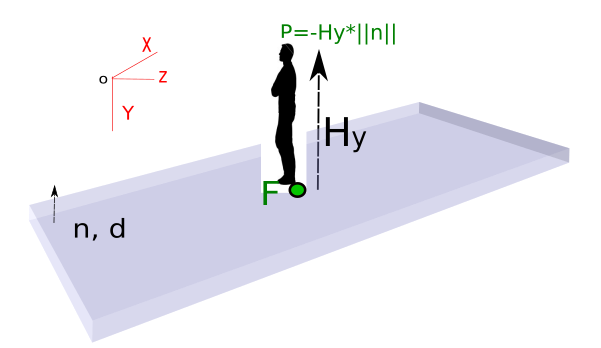
\includegraphics[width=0.5\textwidth]{./pictures/calculoP}
       	\caption{}\label{fig: figura}
      \end{figure}

       \subsubsection{Localización de S}
       Para conocer con precisión cual es la ubicación en pantalla del objeto con respecto a la cámara como marco de referencia con la cámara en cualquier orientación se hizo uso de una unidad Pan-Tilt. Una unidad Pan-Tilt es un dispositivo que permite colocar camáras  en posiciones muy precisas, imagen \ref{pantilt}.\\
          \begin{figure}[htbp]
           	\centering
           	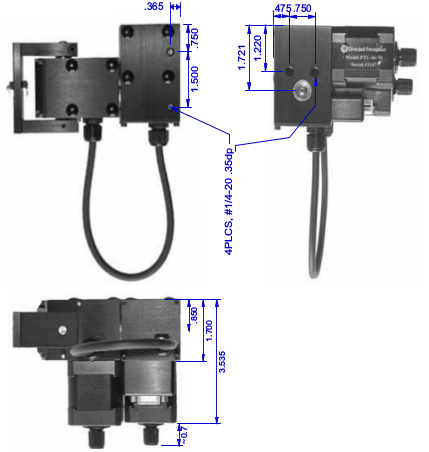
\includegraphics[width=0.2\textwidth]{./pictures/pantilt}
           	\caption{}\label{fig: figura}
           	\label{pantilt}
        \end{figure}
     Sea $O_c$ el eje de rotación de la cámara (punto focal), $O_u$ el eje de rotación de la unidad Pan-Tilt, $D_{cu}$ la distancia en el eje $y$ entre $O_c$ y $O_u$, $\theta$ el ángulo que rota la unidad Pan-Tilt alrededor del eje $X$, $S_1=(S_{1x}, S_{1y}, S_{1z})$ la ubicación inicial de la figura en pantalla antes de la rotación de la unidad y $S_2$ la ubicación después de la rotación, figura \ref{pantilt2} y \ref{pantilt3}. Conociendo $S_1$ con respecto al marco de referencia de la cámara la localización de $S_2$ se realiza tomando en cuenta los parámetros anteriores mediante los siguientes pasos:
              \begin{figure}[htbp]
              	\centering
              	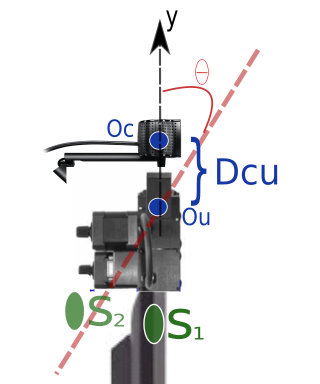
\includegraphics[width=0.3\textwidth]{./pictures/pantilt3}
              	\caption{}\label{fig: figura}
              	\label{pantilt3}
              \end{figure}
      \begin{itemize}
      	\item Colocando la unidad Pan-Tilt con la cámara de manera que el objetivo de la cámara quede de forma perpendicular a la al plano de la pantalla en la cual se proyectarán las figuras que los sujetos de experimentación observarán, lo anterior observando desde el plano $Y-Z$ del marco de referencia.
       \begin{figure}[htbp]
       	\centering
       	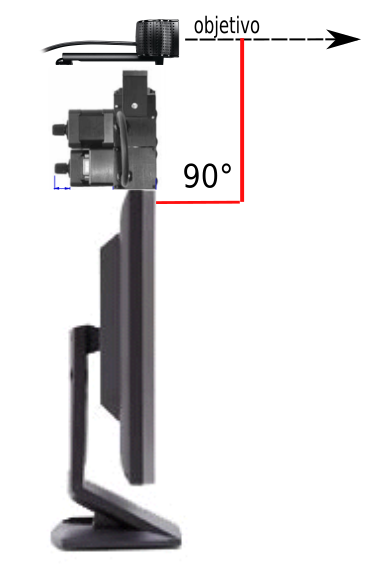
\includegraphics[width=0.2\textwidth]{./pictures/pantilt2}
       	\caption{}\label{fig: figura}
       	\label{pantilt2}
       \end{figure}
      	
      	\item Se traslada el punto $S_1$ hacia el eje de rotación de la cámara $O_c$ mediante $D_{cu}$ metros, únicamente desplazándolo en el eje $Y$.
      	\item Se rota $\theta$ grados el punto a través de la matriz de rotación del eje $X$.
      	\item Finalmente se regresa el punto $D_{cu}$ metros.
      \end{itemize}
	Lo anterior se realiza con la siguiente ecuación:
	%\tiny{		
	        \begin{eqnarray}
	        S_2=
	        \begin{bmatrix}
	        1 & 0 & 0\\
	        0 & cos(-\theta) & -sen(-\theta)\\
	        0 & sen(-\theta) & cos(-\theta)
	        \end{bmatrix}*\begin{bmatrix}S_{1x}\\
	         S_{1y}-D_{cu}\\
	          S_{1z}
	        \end{bmatrix}+\begin{bmatrix}S_{1x}\\
	        S_{1y}+D_{cu}\\
	        S_{1z}
	        \end{bmatrix}
	        \end{eqnarray}
     % }

      
	 \section{Generación de marcas más significativas en el piso y la pantalla} \label{secGen}
	 Como se puede apreciar en el análisis anterior pueden haber infinitas combinaciones de posiciones de marcas en el piso donde se colocan las personas y figuras en la pantalla, inclusive si las regiones en pantalla y piso donde se realiza la captura de datos están limitadas en áreas pequeñas, sin embargo, lo más importante es capturar información en las marcas más relevantes, las cuales son aquellas en las que se da mayor variación en los ángulos de la mirada, es decir, $\phi_x$ y $\phi_y$, esto se hace con el objetivo de que haya variedad en el conjunto de datos de entrenamiento.	\\
	  Al final de esta etapa se genera una secuencia de marcas en el piso en donde a cada una le corresponden dos posiciones diferentes en la pantalla, esto quiere decir que por cada vez que se pare una persona en una marca en el plano del piso se capturará dos veces su rostro en orientaciones diferentes. A continuación se detallará como se realiza el proceso para la selección de los puntos más significativos.	 
	  
	 \subsection{Malla de puntos en el plano del piso y pantalla}
	 De modo que se requiere que la captura de datos (ubicación, ángulos de mirada e imagen) no le lleve bastante tiempo a cada persona, se desarrolló esta etapa con el propósito de que sea automatizada y rápida.
	 El primer paso consiste en generar el arreglo bidimensional de puntos en el plano del piso, es necesario considerar en donde se encuentra el plano del piso en relación al marco de referencia (cámara), por lo tanto se deben tomar en cuenta los parámetros de $n$ y $d$. En base al análisis de los ángulos $\phi_x$ y $\phi_y$ se determina el tamaño del paso en metros en el eje $X$ y $Z$ del piso, y cuales son sus límites máximos y mínimos en ambos ejes. \\
	 Tomando en cuenta lo anterior se genera una matriz de puntos en el piso que representa todas las posiciones posibles en las cuales las personas se pueden colocar para capturar sus datos: $F$, además se calcula para cada posición cual es la ubicación de la cabeza de la persona en la escena: $P$, como se explicó en la sección 4.2.2. Una vez localizada la $P$ se descartan aquellas que no se encuentren en el campo visual de la cámara, ya que de nada sirve capturar una imagen del rostro de la persona si no se encuentra el rostro en ella. Para determinar si el rostro se encuentra en el campo visual de la cámara únicamente se proyecta en la imagen la ubicación de $P$ mediante la matriz de calibración de la cámara, con el resultado obtenido se verifica que esté dentro de los límites visibles de la imagen, si es así, $P$ se encuentra dentro del campo visual de la cámara \\
	 Sea cada punto que representa el rostro $P_1, P_2, P_3...$
	 Sea $P_1$ un punto en el arreglo bidimensional que representa el rostro, se determina cual es el ángulo $\phi_{x1}$ y $\phi_{y1}$ para una figura $S_1$ en la pantalla en una posición fija, a continuación se calcula cual es la rotación de la mirada con respecto a otro punto en la malla: $P_2$ cuyos ángulos son $\phi_{x2}$ y $\phi_{y2}$:
	         \begin{eqnarray}
	         rot_x=\phi_{x1}-\phi_{x2}\\
	         rot_y=\phi_{y1}-\phi_{y2}
	         \end{eqnarray}
	 Lo anterior se calcula para las demás $P$ de la matriz siempre con respecto a $P_1$, al terminar de calcular todas las rotaciones de $P_1$ se pasa a calcular todas las rotaciones de mirada de $P_2$ con todos los demás puntos del arreglo bidimensional. Al final se genera una matriz de matrices de rotaciones de ángulos de la mirada y esto es con respecto a una posición de la figura en pantalla fija, esto es $S_1$.\\
	 En el siguiente paso se generan matrices de matrices para varias ubicaciones de $S$ en pantalla. Después de generar estas matrices, filtrar las rostros: $P$ que presentan mayor variación en rotación y validar que los rostros $P$ se encuentre dentro del campo visual de la cámara se generan las instancias de posibles puntos para capturar datos, cada instancia con el siguiente formato:
	 \begin{eqnarray}
		F1x, F1y, F1z, F2x, F2y, F2z, Sx, Sy, Sz, rot_x, rot_y
	 \end{eqnarray}
	 Los tres primeros datos indican la primera posición en el plano del piso del sujeto de experimento, los siguientes tres datos hacia que punto se movió, los siguientes tres indican la posición de la figura en pantalla para esa instancia y los últimos dos datos señalan la rotación en el vector de la mirada que hubo al pasar de $F1$ a $F2$ con respecto al eje $X$ y al $Y$. 
 
	 \subsection{Generación de secuencia óptima mediante algoritmo de ordenamiento}
	 El algoritmo comienza con la obtención de todas las instancias de rotaciones posibles, es decir la salida de la etapa anterior.
      %Debo detallar más la programación en esta sección?: Clases, funciones
   
       \section{Rotaciones en los pares de posiciones}
       Se eligió como forma de representación de la pose de la cabeza los cuaterniones, los cuales son obtenidos mediante el IMU, como se había mencionado el dispositivo se colocará en la cabeza de las personas durante el entrenamiento para la generación del "ground truth", sin embargo, aún falta considerar los siguientes detalles:
       \begin{itemize}
       	\item ¿Cuáles posiciones en el piso con respecto al marco de referencia centrado en la cámara  se utilizaron para capturar la información(imagen rostro y pose en cuaterniones)?.
       	\item ¿A quá distancia estarán las posiciones entre si y hasta que distancia máxima se tomarán datos, es decir, cual es el mínimo en $X$ y $Z$ que se debe seleccionar? ya que como se observó en la sección de \textit{Análisis del comportamiento de los ángulos $\phi_x$ y $\phi_y$} dependiendo de los parámetros del experimento hay valores en los cuales ya no vale la pena hacer análisis ya que las variaciones en los ángulos es muy pequeño o inexistente.
       	\item ¿Cuáles posiciones para la figura en pantalla se deben utilizar?.
       	\item ¿Cuántas posiciones de figura en pantalla y personas en el piso se considerarán?
       	\item ¿Cómo lidiar con las pequeñas variaciones en las mediciones del IMU que se den en diferentes personas en los mismas instancias de experimentación?
       	
       \end{itemize} 
       
       \subsection{Cálculo de todas las rotaciones posibles}
          \section{Proyección de marcas en el piso}
          Como se mencionó anteriormente para la etapa de entrenamiento del algoritmo de apendizaje automático se debe tener control sobre las capturas que se van a tomar de cada sujeto de experimento incluyendo las posiciones en la escena donde se colocarán al capturar los datos.
          Una vez calculada las mejores posiciones en la escena para capturar los datos con las que se va a entrenar el algoritmo, la siguiente etapa consiste en colocar estos puntos con marcas en el piso para saber durante los experimento en qué posiciones se deben colocar las personas.
          Como se había mencionado las marcas son con respecto al marco de referencia centrado en la cámara, la cual se encuentra sobre la pantalla, dichas marcas se pueden pintar en el piso midiendo sus coordenadas a partir de la cámara mediante un flexómetro o cinta métrica, sin embargo al realizarlo de esta forma se tienen los siguientes problemas:
          \begin{itemize}
          	\item Hay bastante inexactitud, por ejemplo en caso de que no se mida sobre la misma dirección de los ejes debido a pequeños \underline{errores humanos} y esto tiende a agravarse cuando las marcas son lejanas.
          	\item El sistema de coordenadas centrado en la cámara no es paralela al plano del piso donde se colocarán las marcas ya que se debe rotar en dirección al piso para así tener una mejor vista de los rostros de las personas que se encuentran más cercanas a la cámara. Por lo tanto si rotamos la cámara de igual manera rotamos el marco de referencia y es más complicado colocar las marcas, lo anterior se puede ver ilustrado en la figura 11.1. 
          \end{itemize}
          \begin{figure}[htbp]
          	\centering
          	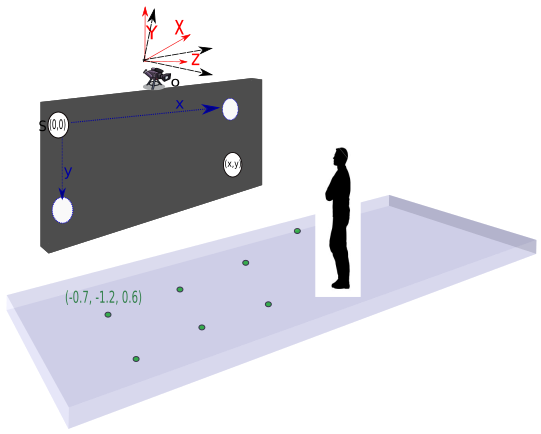
\includegraphics[width=.6\textwidth]{./pictures/ejesRot2}
          	\caption{}\label{fig: figura}
          \end{figure}
          Como solución al problema anterior se desarrollaron algoritmos utilizando visión computacional, geometría y optimización numérica para colocar en el piso de manera más precisa las marcas, el método consiste en conocer cual es la distancia y orientación del plano del piso donde se situarán las personas y  proyectar las marcas en éste tomando como marco de referencia la cámara.
              \subsection{Proyección de marcas mediante visión computacional, geometría y optimización numérica}
              %Se puede explicar a grandes rasgos en que consiste homografía, R y T proyección en el piso y luego detallar
              Para utilizar el método que se describirá a continuación es necesario conocer la matriz de parámetros intrínsecos $K$. La obtención de esta matriz se logró mediante el software de Matlab: Camera Calibration Toolbox, dando como resultado la siguiente matriz.
              \[K=
              \begin{bmatrix}
              fx & 0 & c_x\\
              0 & f_y & c_y\\
              0 & 0 & 1
              \end{bmatrix}
              =
              \begin{bmatrix}
              616.164 & 0 & 325.528\\
              0 & 616.82 & 228.66\\
              0 & 0 & 1
              \end{bmatrix}
              \]
       \subsubsection{Homografía}
       Durante la primera etapa se debe hallar la homografía que mapea puntos en el plano del piso y los respectivos puntos en la imagen de ese plano, todas coordenadas deben estar en metros, los puntos en el plano del piso deben tener las medidas reales que hay entre ellos, tener uno de los puntos como origen y con respecto a éste establecer las coordenadas de las demás.\\
       La matriz de homografía se descompone y a partir de ella se encuentra la matriz de rotación y el vector de traslación que existe entre el plano del piso y la cámara, es decir, este método se basa en un modelo conocido 3D y su correspondencia en el plano imagen 2D.\\
       Inicialmente se creó un software para capturar con el mouse 4 puntos marcados en el piso siguiendo un orden en específico, la matriz con los puntos establecidos con las medidas reales se denomina $scnPts_{4x4}$ y la matriz obtenida con los puntos capturados con el mouse se denomina $imgPts_{3x4}$. Los puntos establecidos en el piso tienen forma cuadrangular y están separados entre sí a $0.4m$, tomando como origen el punto de la esquina superior izquierda y como primera captura, como segundo punto la esquina inferior izquierda, tercer punto la esquina inferior derecha y último la esquina superior derecha establecemos la siguiente matriz:
       \[scnPts=
       \begin{bmatrix}
       0 & 0 & 0.4\\
       0 & 0.4 & 0.4\\
       0 & 0 & 0\\
       1 & 1 & 1 
       \end{bmatrix}
       \]
       donde cada columna es un punto, la primera fila representa la coordena en el eje $x$, la segunda en $y$ y la tercera en $z$. Nótese que son coordenadas homogéneas y el valor en $z$ es cero ya que todos los puntos yacen sobre el mismo plano. Como se puede observar la matriz $scnPts$ está en metros por lo tanto se requiere que $imgPts$ igual esté en metros, esto se consigue simplemente multiplicando la matriz $imgPts$ por la inversa de la matriz $K$.\\
       Como resultado del proceso anterior se obtuvo una homografía inexacta ya que al comprobar si mapeaba los puntos de la escena a la imagen ésta no lo hacía correctamente, los puntos tenían bastante error.
       El error en la matriz de homografía podría deberse a los siguientes motivos:
       \begin{itemize}
       	\item  Hay una distancia considerable entre los puntos del plano y la imagen
       	\item La captura de los puntos en la imagen mediante el mouse es realizada por simple inspección y seleccionando los puntos lo cual podría generar capturas erróneas.
       	\item Son pocos puntos para calcular la homografía
       \end{itemize}
       Para solucionar los inconvenientes anteriores se optó por utilizar más puntos, para ello se colocó una manta con un tablero de ajedrez con 48 intersecciones o en este caso 48 puntos con una longitud de $12cm$ cada lado, esto quiere decir que los puntos estarán separados a $0.12m$, además con el objetivo de que sea más precisa la captura y automática se modificó el programa para localizar las intersecciones automáticamente mediante bibliotecas de openCV y no estar capturando manualmente los puntos. Ahora la matriz $scnPts$ tiene una dimensión de $4x48$ y imgPts $3x48$. En la imagen 11.2 se pueden notar el buen desempeño que tiene algoritmo al encontrar las intersecciones en la manta con el tablero de ajedrez.
       \begin{figure}[htbp]
       	\centering
       	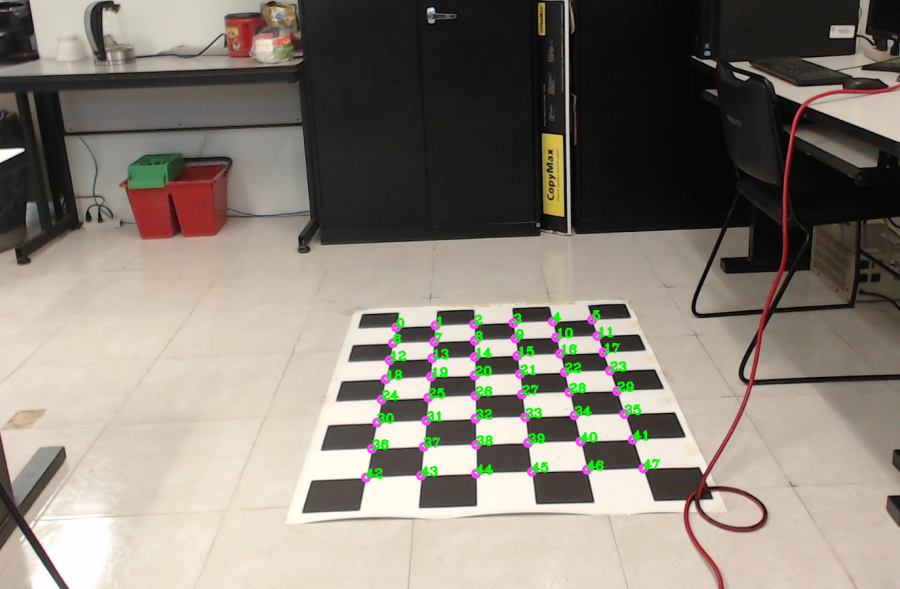
\includegraphics[width=.6\textwidth]{./pictures/ajedrez}
       	\caption{}\label{fig: figura}
       \end{figure}
       
       \subsubsection{Rotación y traslación de la cámara}
       Con la homografía $H$ se calcula la pose de la cámara (matriz de rotación $R_{3x3}$ y vector de traslación $T_{3x1}$) con respecto al plano del piso, además, se puede calcular la ecuación del plano la cual será útil más adelante.\\
       \[H=
       \begin{bmatrix}
       h_{11} & h_{12} & h_{13}\\
       h_{21} & h_{22} & h_{23}\\
       h_{31} & h_{32} & h_{3}\\
       \end{bmatrix}
       \]          
       	La primera columna de $H$ contiene la primera columna de $R$ ($R_1$), es decir, la rotación al rededor del primer eje, la segunda columna es la segunda columna de $R$ ($R_2$) y la tercera columna de $H$ es el vector de traslación $T$, solamente queda por calcular la tercera columna de $R$ ($R_3$) la cual tiene que ser ortogonal a las dos primeras, por lo tanto se puede calcular mediante el producto cruz de la primera columna de h con la segunda. Adicionalmente antes de calcular la tercera columna de la matriz de rotación es necesario normalizar $R$ y $T$ debido a redundacias. La normalización se realiza de la siguiente manera:
       	\begin{eqnarray}
       	norm1=||[h_{11} h_{21} h_{31}]^T||\\
       	norm2=||[h_{12} h_{22} h_{32}]^T||\\
       	normT=\frac{norm1+norm2}{2}			
       	\end{eqnarray}
       	\[R=
       	\begin{bmatrix}
       	\frac{h_{11}}{norm1} & \frac{h_{12}}{norm2} & R_{13}\\
       	\frac{h_{21}}{norm1} & \frac{h_{22}}{norm2} & R_{23}\\
       	\frac{h_{31}}{norm1} & \frac{h_{32}}{norm2} & R_{33}\\
       	\end{bmatrix}
       	, T=
       	\begin{bmatrix}
       	\frac{T_x}{normT}\\
       	\frac{T_y}{normT}\\
       	\frac{T_z}{normT}	
       	\end{bmatrix}
       	\]
       	Luego simplemente se aplica el producto cruz para obtener la tercera columna
       	\begin{eqnarray}
       	R_3=R_1 \otimes R_2
       	\end{eqnarray}
       	Para hallar la ecuación del plano con respecto a la cámara (marco de referencia): $Ax+By+Cz=d$ únicamente es necesario la $R$, $T$ de la cámara y un punto de la escena de los que se utilizaron para el cálculo de la homografía.
       	\subsubsection{Cálculo de la ecuación del plano}
       	Como es bien sabido la normal  $n$ al plano $\Pi$ está dado por los componentes: $A$, $B$ y $C$ de la ecuación del plano y la distancia más cercana del plano al origen por: $d$, figura
       	
       	\begin{figure}[htbp]
       		\centering
       		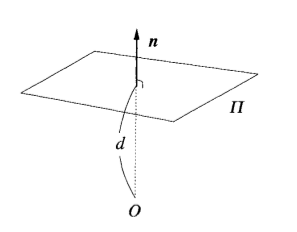
\includegraphics[width=.4\textwidth]{./pictures/plane}
       		\caption{Representación de un plano en el espacio}\label{fig: figura}
       	\end{figure}
       	Tomando como marco de referencia el plano (puntos establecidos en $scnPts$) la normal está dada por el eje $Z$ por lo tanto para obtener la normal con respecto al marco de referencia en la cámara unicamente rotamos este vector con la matriz de rotación:
       	\[n=R*\begin{bmatrix}
       	0\\
       	0\\
       	1	
       	\end{bmatrix}\]
       	Sea $scnPts1_{3x1}$ el primer punto de la matriz de puntos establecidos en la escena, entonces la distancia $d$ del plano al origen es este punto rotado y trasladado hacia la cámara, y al resultado se le aplica el producto punto con la normal al plano:
       	\begin{eqnarray}
       	scnPtsRot=R*scnPts1+T\\
       	d=<N,scnPtsRot>
       	\end{eqnarray}
       	
       	\subsubsection{Reproyección de puntos en la imagen} \label{repPtsIm}
       	Todo el proceso anterior se realiza con el objetivo de poder proyectar puntos en la imagen sobre el plano del piso tomando como marco de referencia la cámara. Lo anterior se consigue únicamente estableciendo la matriz con las marcas en el piso que se necesitan y proyectándolas en la imagen multiplicando por la matriz de parámetros intrínsecos para pasar las coordenadas a pixeles.\\
       	Antes de pasar a esa etapa es necesario verificar que los parámetros encontrados en la sección anterior: $R$, $T$, $n$ y $d$ son correctos. 
       	\begin{itemize}
       		\item La verificación de $n$ y $d$ consiste en utilizar los puntos obtenidos de $imgPts$ y proyectarlos desde el origen hacia el plano (formando rectas) y encontrar las coordenadas en las cuales se intersectan dichas proyecciones con el plano, estas intersecciones deben ser las mismas que las coordenadas de $scnPts$. Sea $L$ la recta en el espacio, $rh$ el vector que va del punto más cercano de $L$ al origen y $m$ el vector unitario que indica la orientación de $L$. 
       		\begin{figure}[htbp]
       			\centering
       			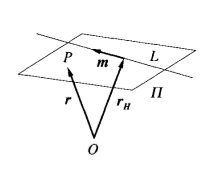
\includegraphics[width=.35\textwidth]{./pictures/intersec}
       			\caption{intersección de una recta con un plano}\label{fig: figura}
       		\end{figure}
       		
       		La intersección de $L$ con el plano $\Pi$ en $r$ está dada por:
       		\begin{eqnarray}
       		r=r_H+\frac{d-<n_{\Pi}, r_H>}{<n_{\Pi},m>}m
       		\end{eqnarray}
       		En este caso las lineas (proyecciones de imgPts) parten de la cámara por lo tanto el vector $rh$ es igual cero, simplificando la ecuación la intersección queda de la siguiente manera:
       		\begin{eqnarray}
       		r=\frac{d}{<n_{\Pi},m>}m
       		\end{eqnarray}	
       		
       		\item La verificación de $R$ y $T$ simplemente se realiza tomando los puntos de $scnPts$ rotándolos, trasladándolos y proyectándolos en la imagen, en caso de que los cálculos de la $R$ y $T$ sean correctos estas proyecciones deben ser las mismas que $imgPts$.
       	\end{itemize}

       	
       	\subsection{Optimización Levenberg-Marquardt} \label{opNum}
       	Como se mencionará más adelante en la etapa experimental la rotación y traslación no son lo suficientemente precisas para empezar a realizar experimentos. Por lo tanto se opta por utilizar un algoritmo de optimización numérica para minimizar el error que existe en la rotación y traslación. Se eligió el algoritmo de Levenberg-Marquardt debido a que es uno de los más eficientes, con él se busca el vector de parámetros $p$ que minimice.
       	
       	%en uno de los peores casos hay una diferencia de $26cm$ con la coordenada sobre el eje $X$ que debiera ser. 
       	\begin{eqnarray}
       	F(p)=\frac{1}{2}\sum\limits_1^m(f_i(p))^2	
       	\end{eqnarray}
       	donde $f: \mathbb{R}^n\rightarrow \mathbb{R}, i=1,....,m$ son las funciones dadas y $m\geq n$.     	
       	Las funciones a optimizar deben tener los parámetros de $R$ y $T$, estar descritas de tal forma que sean iguales o cercanas a cero, e incluir a los 48 puntos, por lo tanto el número de ecuaciones a minimizar es $m=144$ (tomando en cuenta los tres componentes de cada punto) y se plantean de la siguiente forma:
       	\begin{eqnarray}
       	f_{xyz}(p)=||X_{rt}-X_{intersec}||
       	\end{eqnarray}
       	donde $X_{rt}$ es el conjunto de puntos $scnPts$ rotados y trasladados, y $X_{intersec}$ es el conjunto de puntos $imgPts$ que se proyectan e intersectan con el plano. Por cada conjunto de tres ecuaciones se tiene:
       	\begin{eqnarray}
       	f_{xyz}(p)= \{R*X_{scn}+T\}-\{ \frac{d}{<n_{\Pi},X_{img}>}X_{img} \}
       	\end{eqnarray}
       	Como se explicó anteriormente la $n$ y $d$ del plano dependen de la rotación y traslación por lo que es importante también ir actualizando estos parámetros en cada paso de la optimización. \\
       	%No es congruente estar optimizando los 9 parámetros de la matriz de rotación, esto puede generar errores 
       	En problemas de optimización numérica la redundancia de las matrices de rotación es inconveniente y a menudo es preferible una representación mínima. La representación más simple la cual está basada en el teorema de Euler dice que cada rotación puede ser descrita por un eje de rotación y un ángulo alrededor de él. Una compacta representación del eje y el ángulo es un vector de rotación de tres dimensiones cuya dirección es el eje y cuya magnitud es el ángulo en radianes.\\
       	%La fórmula de rotación de Rodrigues puede ser usada para transformar todo los ve
       	Por lo que se optimizará el eje de rotación y su magnitud del ángulo de rotación, ya que como indica la fórmula de Rodrigues cualquier matriz de rotación se puede realizar mediante la rotación alrededor de un eje fijo $\omega$ por un cierto ángulo $\parallel\omega\parallel$:
       	\begin{eqnarray}
       	R=I+\frac{\hat{\omega}}{\parallel\omega\parallel}sin(\parallel\omega\parallel)+ \frac{\hat{\omega}^2}{\parallel\omega\parallel^2}(1-cos(\parallel\omega\parallel))
       	\end{eqnarray}
       	Donde los valores del eje y el ángulo de una matriz $R$:
       	\[R=
       	\begin{bmatrix}
       	r_{11} & r_{12} & r_{13}\\
       	r_{21} & r_{22} & r_{23}\\
       	r_{31} & r_{32} & r_{33}\\
       	\end{bmatrix}
       	\]
       	se obtienen por medio de:
       	\begin{eqnarray}
       	\parallel\omega\parallel=cos^{-1}  \lgroup \frac{traza(R)-1}{2}\rgroup, \frac{\omega}{\parallel\omega\parallel}=\frac{1}{2sin(\parallel\omega\parallel)} \begin{bmatrix}
       	r_{32}-r_{23}\\
       	r_{13}-r_{31}\\
       	r_{21}-r_{12} \\
       	\end{bmatrix}	
       	\end{eqnarray}
       	
       	Los 7 parámetros optimizar son los siguientes:
       	\begin{eqnarray}
       	\begin{array}{c}
       	p=[\omega_x, \omega_y, \omega_z, \parallel\omega\parallel, T_x, T_y, T_z]
       	\end{array}
       	\end{eqnarray}
       	En el algoritmo de levenberg-marquardt se debe definir cuales son cada una de las funciones y no es suficiente con 48 ecuaciones como la de 11.10 ya que ésta involucra multiplicaciones de matrices de 3 filas (son conjuntos de puntos de 3 coordenadas) teniendo en realidad 144 funciones a optimizar. Por lo tanto es necesario expresar la ecuación 11.10 en términos de $\omega_x, \omega_y, \omega_z, \parallel\omega\parallel, T_x, T_y, T_z$ con ayuda de la fórmula de Rodrigues para poder utilizar el algoritmo de optimización. Por lo que para cada una de las $x$ de las 48 de la ecuación 11.10 de $X_{rt}$ (la parte de $X_{intersec}$ está más claro como usarla debido a la ecuación 11.11) la función de optimización es:
       	%	\begin{equation}
       	%	\resizebox{1.2\hsize}{!}{$%
       	%	f_{xi}(p)= \{[(\omega_x^2-1)(1-cos(\parallel\omega\parallel))+1]X_{scnxi}+ [\omega_x\omega_y(1-cos(\parallel\omega\parallel))-\omega_z(sin(\parallel\omega\parallel))]X_{scnyi}+[\omega_ysin(\parallel\omega\parallel)+\omega_x\omega_z(1-cos(\parallel\omega\parallel))]X_{scnzi}\}+T_x 
       	%	$%
       	%	}%
       	%	\end{equation}
       	
       	\begin{eqnarray}
       	\begin{array}{c}
       	f_{xi}(p)=[(\omega_x^2-1)(1-cos(\parallel\omega\parallel))+1]X_{scnxi}+\\
       	\qquad \qquad \qquad  \left[\omega_x\omega_y(1-cos(\parallel\omega\parallel))-\omega_z(sin(\parallel\omega\parallel))\right]X_{scny}+\\
       	\qquad \qquad \qquad \qquad
       	\left[\omega_ysin(\parallel\omega\parallel)+\omega_x\omega_z(1-cos(\parallel\omega\parallel))\right]X_{scnzi}\}+T_x 
       	\end{array}
       	\end{eqnarray}
       	
       	Para cada una de los puntos en y de los 48 la función de optimización es:
       	%		\begin{equation}
       	%		\resizebox{1.2\hsize}{!}{$%
       	%		f_{yi}(p)=[\omega_zsin(\parallel\omega\parallel)+\omega_x\omega_y(1-cos(\parallel\omega\parallel))]X_{scnxi}+
       	%		[(\omega_y^2-1)(1-cos(\parallel\omega\parallel))+1]X_{scnyi}-
       	%		[\omega_xsin(\parallel\omega\parallel)+\omega_y omega_z(1-cos(\parallel\omega\parallel))]X_{scnzi}+T_y
       	%	$% 
       	%	}%
       	%\end{equation}	
       	\begin{eqnarray}
       	\begin{array}{c}
       	f_{yi}(p)=[\omega_zsin(\parallel\omega\parallel)+\omega_x\omega_y(1-cos(\parallel\omega\parallel))]X_{scnxi}+\\
       	\left[(\omega_y^2-1)(1-cos(\parallel\omega\parallel))+1\right]X_{scnyi}-\\
       	\qquad \qquad \qquad \qquad
       	\left[\omega_xsin(\parallel\omega\parallel)+\omega_y omega_z(1-cos(\parallel\omega\parallel))\right]X_{scnzi}+T_y
       	\end{array}
       	\end{eqnarray}
       	
       	Finalmente en los puntos pertenecientes a la coordenada z la función es:
       	%		\begin{equation}
       	%		\resizebox{1.2\hsize}{!}{$%
       	%		f_{zi}(p)=[\omega_x\omega_z(1-cos(\parallel\omega\parallel))-\omega_y\sin(\omega)]X_{scnxi}+
       	%		[\omega_xsin(\parallel\omega\parallel)+\omega_y\omega_z(1-cos(\parallel\omega\parallel))]X_{scnyi}+
       	%		[(\omega_z^2-1)(1-cos(\parallel\omega\parallel))+1]X_{scnzi}+T_z
       	%		$% 
       	%		}%
       	%		\end{equation}
       	\begin{eqnarray}
       	\begin{array}{c}
       	f_{zi}(p)=[\omega_x\omega_z(1-cos(\parallel\omega\parallel))-\omega_y\sin(\omega)]X_{scnxi}+\\
       	\qquad \qquad
       	\left[\omega_xsin(\parallel\omega\parallel)+\omega_y\omega_z(1-cos(\parallel\omega\parallel))\right]X_{scnyi}+\\
       	\qquad	
       	\left[(\omega_z^2-1)(1-cos(\parallel\omega\parallel))+1\right]X_{scnzi}+T_z
       	\end{array}
       	\end{eqnarray}
 
\section{Red neuronal}
    El algoritmo clasificador propuesto para esta etapa de la tesis es una red neuronal de propagación hacia atrás, donde las neuronas de entrada es el vector de características y las neuronas de salida representan región en la pantalla que se observa, a continuación se describe como se implementa la red neuronal en el presente proyecto comenzando con el tratamiento de datos incluidas las imágenes para representarlos como el vector de características.
	\begin{figure}[htbp]
		\centering
		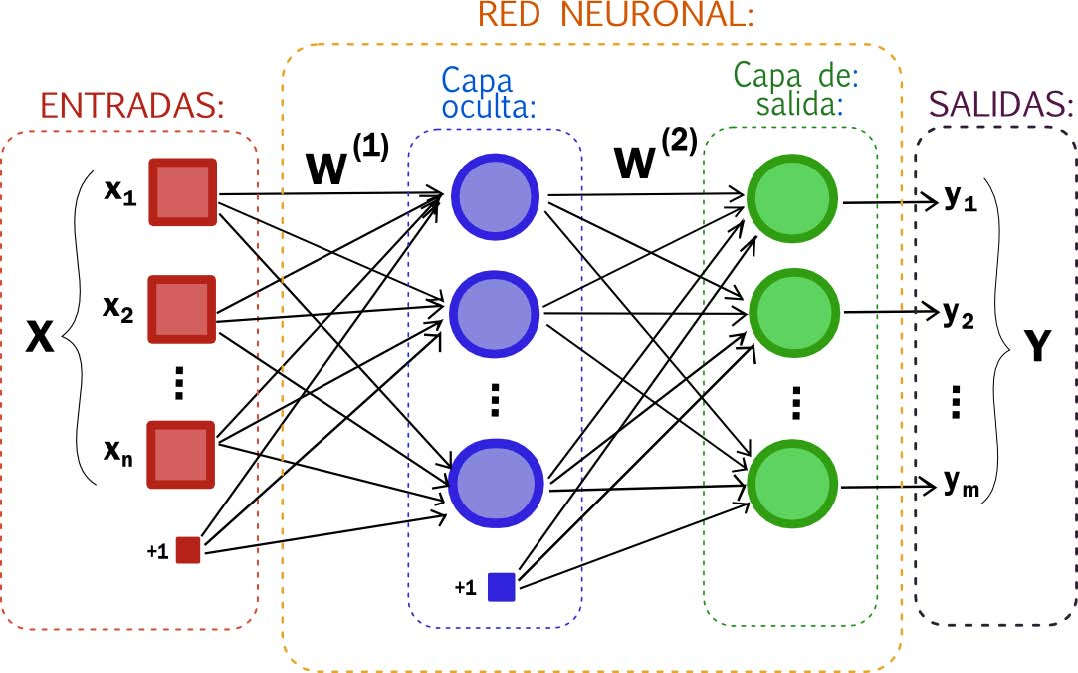
\includegraphics[width=.5\textwidth]{./pictures/neuralNet}
		\caption{Red neuronal artificial}\label{fig: figura}
	\end{figure}
	
\subsection{Vector de características de entrada}\label{inFeature}
	Con las imágenes y la información capturada se preparan los datos para la red neuronal, para ello se generan dos etapas de tratamiento de datos, la primera consiste de los siguientes pasos:
	\begin{enumerate}
		\item Se procesan cada una de las imágenes capturadas con el algoritmo de Viola y Jones para la detección de rostros
		\item De las imágenes con rostros detectados se extrae la región en la imagen donde se encuentra el rostro mediante un ROI.
		\item El ROI de la cara de la persona se guarda para posterior análisis junto con los datos de ubicación 3d en las escena del rostro y la ubicación (igual 3d) de lo que estaba observando en pantalla al momento de la captura, esto es: $P$ y $S$
		\item Finalmente se acompleta la información con la resolución original del ROI del rostro ya que en una etapa posterior es necesario redimensionar todos los rostros a una misma resolución.
	\end{enumerate}
	La salida de este proceso tiene por cada rostro un conjunto de 8 datos los cuales son: \textit{la imagen, la dimensión original del rostro}, $P_x$, $P_y$, $P_z$, $S_x$, $S_y$, $S_z$. Utilizar la resolución original del ROI del rostro como una característica del vector, sirve como una indicador de la distancia sobre el eje $Z$ de la persona, más adelanta en la etapa experimental se entrarás más en detalle.
		\begin{figure}[htbp]
			\centering
			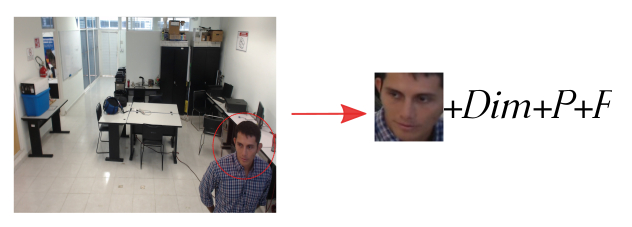
\includegraphics[width=.6\textwidth]{./pictures/featureNet}
			\caption{Características}\label{fig: figura}
		\end{figure}
	\\La segunda etapa consiste simplemente en acomodar los datos resultantes del proceso anterior en forma del vector de características que se requiere en las neuronas de entrada de la red. En cada ejemplo de entrenamiento se redimensiona la imagen del rostro a un estándar $dimE$ para todos, en donde cada pixel representa una característica del vector. Por lo tanto al final se obtiene el vector de características con $dimE+4$ elementos, donde los 4 restantes elementos son la dimensión original del rostro y $P$.
	%Añadir imagen que represente como cada pixel se le asocia una neurona en la entrada
	
\subsection{Neuronas de salida}
En este proyecto cada neurona de salida representa una partición de la pantalla que la persona está observando, esto quiere decir que si por ejemplo si solamente se tienen dos neuronas de salida la pantalla será particionada en dos regiones, durante la etapa experimental se experimentará con diferentes topologías de la red y número de neuronas de salida.
Con respecto a lo anterior es necesario mapear la figura de lo que observa la persona $S$ (etiqueta) a una neurona de salida, ya que se conocen las dimensiones de la pantalla donde se desplaza $S$, en consecuencia únicamente se determina en que región de la pantalla se encuentra $S$ para cada ejemplo de entrenamiento y se le coloca un uno a esa neurona, en caso contrario se coloca un cero, figura \ref{fig: outNeu}.
		\begin{figure}[htbp]
			\centering
			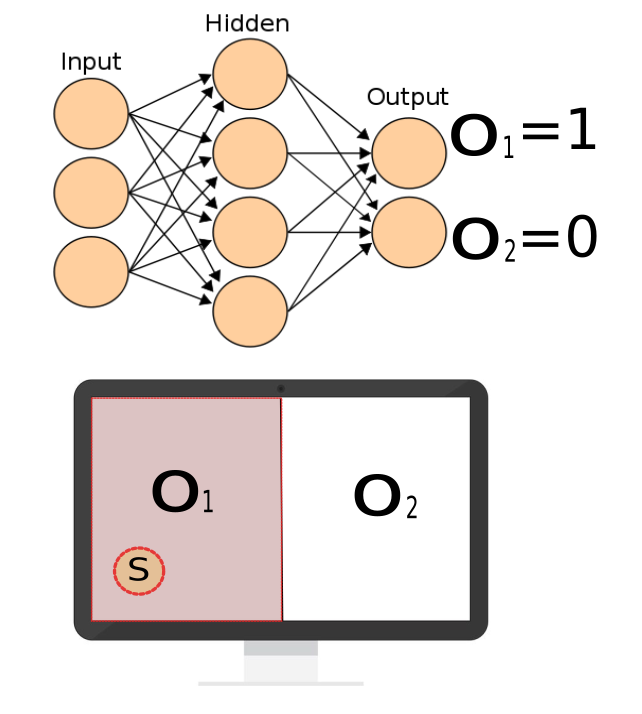
\includegraphics[width=.5\textwidth]{./pictures/outNeu}
			\caption{Neuronas de salida}\label{fig: outNeu}
		\end{figure}